%% Requires compilation with XeLaTeX 
\documentclass[10pt,xcolor={table,dvipsnames},t]{beamer}
\usetheme{UCBerkeley}
\usefonttheme[onlymath]{serif}

\usepackage{graphics,graphicx,float}
\usepackage{multicol}
\usepackage{cancel}
\usepackage[export]{adjustbox}

\hypersetup{pdfstartview={Fit}}

\title{CP Violation In and Beyond The Standard Model}
\subtitle{Two Higgs Doublet Model Type II Contributions to Flavour Observables}
\author{Matthew Rossetter}
\institute{}
\date{\today}

\graphicspath{{../images/}}

\begin{document}

\section{Introduction}
\begin{frame}
  \titlepage
\end{frame}

% Uncomment these lines for an automatically generated outline.
%\begin{frame}{Outline}
%  \tableofcontents
%\end{frame}
\begin{frame}{The Standard Model}
    \begin{itemize}
        \item One of the great achievements of the 20th Century, the Standard Model:
            \begin{align*}
                \mathcal{L} &= \underbrace{-\frac14 F_{\mu\nu}F^{\mu\nu}}_{\text{\small gauge fields}} \underbrace{+ i\bar{\Psi}\cancel{D}\Psi}_{\text{\small fermions}} \underbrace{+ (D_\mu\Phi)^\dagger(D^\mu\Phi) - V(\Phi)}_{\text{\small Higgs}} \underbrace{- Y_{ij}\bar{\Psi}_i\Phi\Psi_j + h.c.}_{\text{\small Yukawa}}
            \end{align*}
        \item A gauge field theory describing matter and its interactions with 25 fundamental particles
        \item Each particle is described by a field transforming under the gauge groups of the Standard Model: SU(3)$_c\otimes$SU(2)$_L\otimes$U(1)$_Y$
        \item Has successfully described numerous particle phenomena we have observed to date
    \end{itemize}
\end{frame}

\begin{frame}{Unsolved Problems of the Standard Model}
    \begin{itemize}
        \item Quantum gravity; Dark matter; Neutrino masses
        \item Deviations between experiment and theory, e.g. $\mathcal{R}(K^{(*)})$ to $\approx3\sigma$ %https://arxiv.org/pdf/2002.12910.pdf
        \item Sakharov Criteria for Baryogenesis:
            \begin{enumerate}
                \item Baryon Number Violation - theorised in Sphalerons
                \item C and CP Violation - present but not enough
                \item First Order Phase Transition - only if $m_h<60\,$GeV 
            \end{enumerate}
    \end{itemize}
    To answer these questions, we need to consider models to extend our physics Beyond the Standard Model. 
    These models should:
    \begin{itemize}
        \item preserve predictions in agreement with experiment
        \item agree with experimental bounds
        \item follow the structures of gauge field theory for a physical model, e.g. renormalisability
    \end{itemize}
\end{frame}

\begin{frame}{The Two Higgs Doublet Model Type II}
    \begin{columns}[t]
        \begin{column}{0.5\textwidth}
            In the Standard Model:
            \begin{itemize}
                \item One complex Higgs doublet, 4 scalar fields:
                    \begin{align*}
                        \Phi_1 &= \begin{pmatrix} \phi_1 + i\phi_2 \\ \phi_0+i\phi_3\end{pmatrix}
                    \end{align*}
                \item 3 fields ``eaten" by $W^\pm,Z$ bosons;\\ 1 real field left, $h$
                \item Introduce $\tilde{\Phi}=i\sigma_2\Phi_1$ for masses of all fermions
            \end{itemize}
        \end{column}
        \begin{column}{0.5\textwidth}
            In 2HDM:
            \begin{itemize}
                \item Add a second doublet, now 8 scalar fields
                    \begin{align*}
                        \Phi_2 &= \begin{pmatrix} \phi_5 + i\phi_6 \\ \phi_4 + i \phi_7\end{pmatrix}
                    \end{align*}
                \item Now 5 fields left - $H^\pm,H^0,h^0,A^0$
                \item No need for Hermitian conjugate
                \item In Type II, $\Phi_1$ couples to down quarks; $\Phi_2$ to up quarks and charged leptons
            \end{itemize}
        \end{column}
    \end{columns}
\end{frame}

\begin{frame}{Why Two Higgs Doublet Model?}
    \begin{itemize}
        \item Minimal Extension to SM
        \item Limited number of new parameters:
            \begin{itemize}
                \item Masses of $H^\pm,H^0,A^0$; VEV ratio $\tan\beta=\frac{v_2}{v_1}$; scalar mixing angle
            \end{itemize}
        \item Sakharov Criteria:
            \begin{enumerate}
                \item Baryon Number Violation - Sphalerons
                \item C and CP violation - more of it
                \item First Order Phase Transition - now present
            \end{enumerate}
        \item Charged weak currents gain additional decay paths, replacing $W^\pm$ with $H^\pm$ - allows for easy constraining
    \end{itemize}
    \begin{figure}[H]
        \centering
        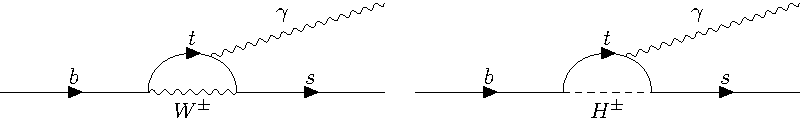
\includegraphics[scale=0.6]{../presentation/fine1.pdf}
    \end{figure}
\end{frame}

\section{Global Fits}
\begin{frame}{First Inputs}
    \begin{columns}[T]
        \begin{column}{0.33\textwidth}
            \vspace{1.5em}
            \begin{itemize}
                \item $1\sigma$ scan
                \item Leptonic, mixing, and radiative
                \item No hard constraint on $\tan\beta$
                \item $m_{H^+} > 340\,$GeV
            \end{itemize}
        \end{column}
        \begin{column}{0.60\textwidth}
            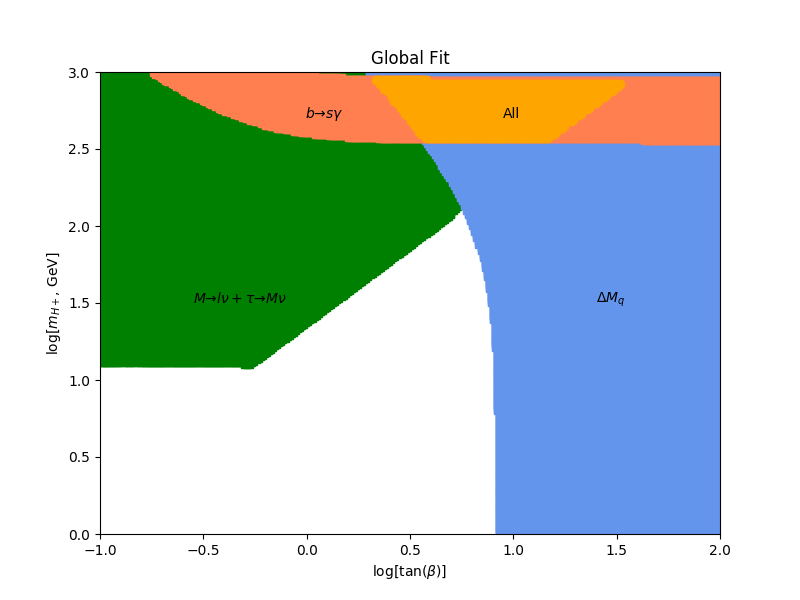
\includegraphics[scale=0.35]{global}
        \end{column}
    \end{columns}
\end{frame}
            %Initial stuff from 0907.5135 here.
\begin{frame}{Statistical Fitting of Scans}
    \begin{columns}[T]
        \begin{column}{0.4\textwidth}
            \begin{itemize}
                \item Aimed to replicate process of original paper (see below) 
                \item Used 2009 inputs
                \item Scanned at 95\% CL
                \item $\chi^2$ fit to $1\sigma$
                \item Replicated $m_{H^+}\gtrapprox316\,$GeV, 95\% CL
            \end{itemize}
        \end{column}
        \begin{column}{0.55\textwidth}
            \vspace{-1.5em}
            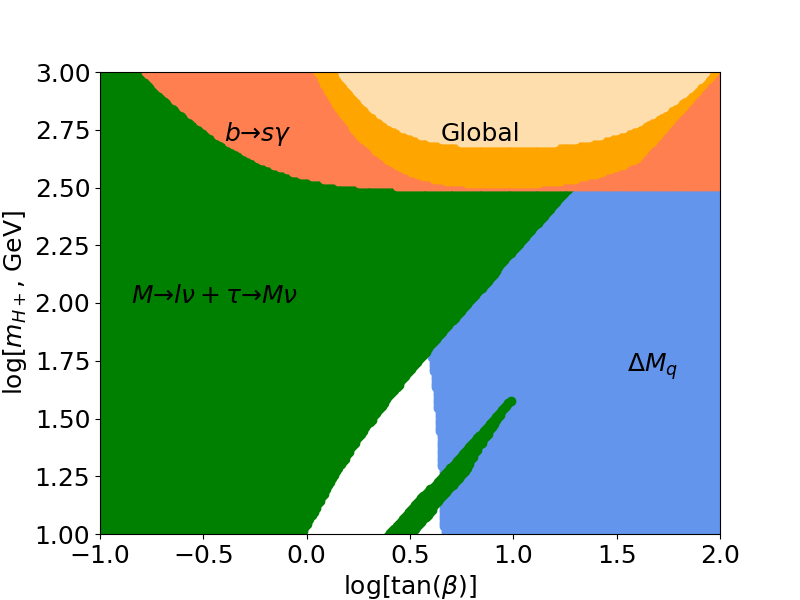
\includegraphics[scale=0.35]{global_08}
        \end{column}
    \end{columns}
    \emph{\small O Deschamps et al, Phys. Rev. D82 (2010) 073012, arxiv:0907.5135 [hep-ph]}
\end{frame}

\begin{frame}{New Inputs}
    \begin{columns}[c]
        \begin{column}{0.45\textwidth}
            \begin{itemize}
                \item $B_s\to\mu^+\mu^-$ 
                    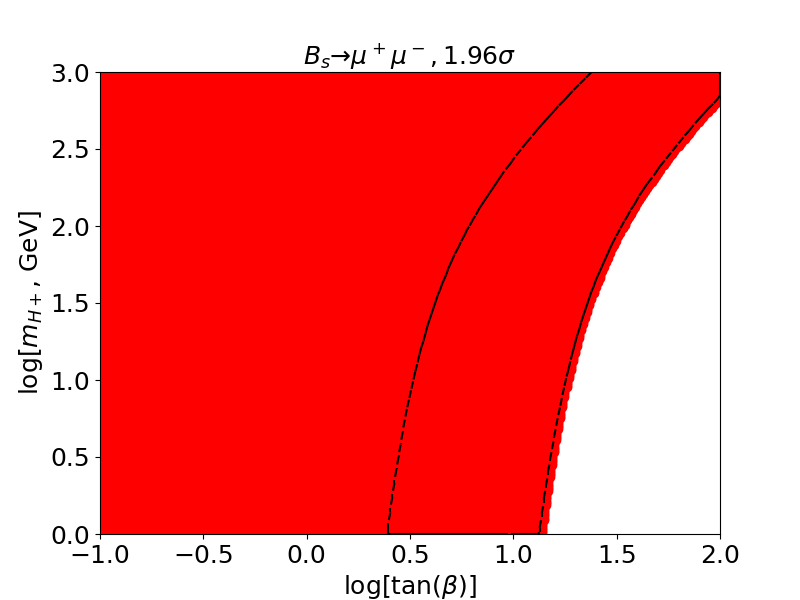
\includegraphics[scale=0.25]{mumu}
            \end{itemize}
        \end{column}
        \begin{column}{0.45\textwidth}
            \begin{itemize}
                \item $R(D^{(*)}) = \frac{\Gamma[B\to D^{(*)}\tau\nu]}{\Gamma[B\to D^{(*)}l\nu]}$ 
                    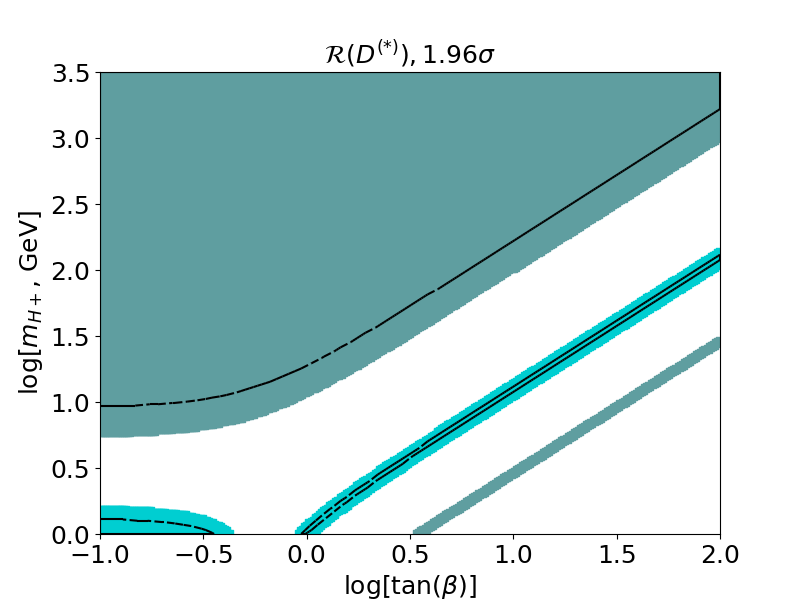
\includegraphics[scale=0.25]{rd_95both}
            \end{itemize}
        \end{column}
    \end{columns}
    \begin{itemize}
        \item 2HDM historically struggles fitting both $\mathcal{R}(D)$ and $\mathcal{R}(D^*)$
        \item Does this kill the 2HDM?
    \end{itemize}
\end{frame}

\begin{frame}{Extended Global Fit}
    \begin{columns}[T]
        \begin{column}{0.37\textwidth}
            \vspace{1.5em}
            \begin{itemize}
                \item Added $B_s\to\mu^+\mu^-$ and $\mathcal{R}(D)$
                \item $\mathcal{R}(D^*)$ not included
                \item 95\% CL: $m_{H^+}>390\,$GeV
                \item $1\sigma$: $m_{H^+}>530\,$GeV
                \item $\tan\beta\gtrapprox2$
            \end{itemize}
        \end{column}
        \begin{column}{0.60\textwidth}
            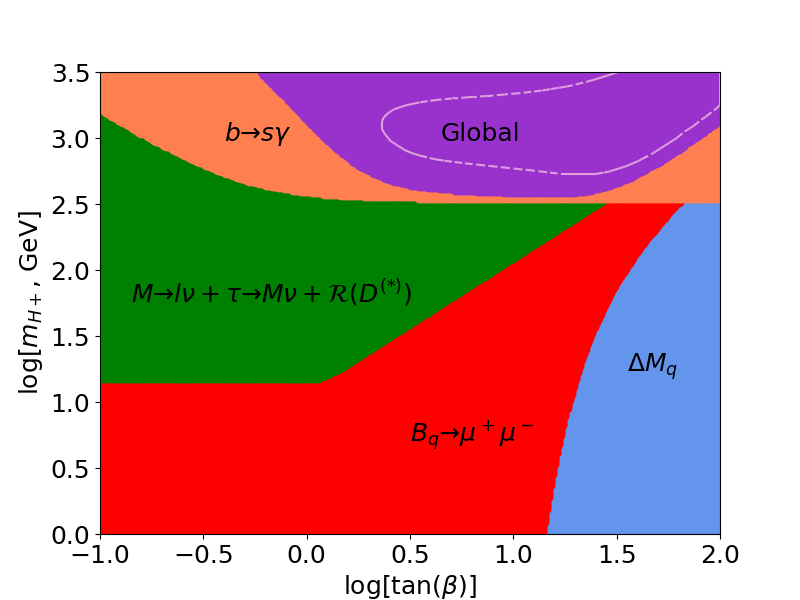
\includegraphics[scale=0.35]{global_lines.png}
        \end{column}
    \end{columns}
\end{frame}

\begin{frame}{CKM Element Modifications}
    \begin{itemize}
        \item CKM Matrix contains information of quark mixing 
        \item In SM, a $3\times3$ unitary matrix
        \item Measurements would be modified in 2HDM as
            \begin{align*}
                V_{ij} &= \frac{V_{ij}^{SM}}{f^{SM}+f^{2HDM}}, & 
                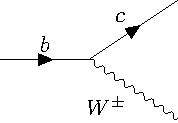
\includegraphics[width=0.25\textwidth,valign=c]{bcw.pdf} &+ 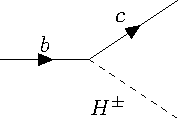
\includegraphics[width=0.25\textwidth,valign=c]{bch.pdf}
            \end{align*}
        \item Exclusive measurements from light quark mesons would have negligible change, but heavy quarks could introduce significant changes
        \item Possibility to improve unitarity constraints, e.g. second row currently sums to $>1$
%        \item Space for a fourth generation? %1172, 46
    \end{itemize}
\end{frame}

\section{Extension to SM4}
\begin{frame}{Four Generations?}
    \begin{block}{Why SM4?}
        \begin{itemize}
            \item $3\times3$ CKM $\to4\times4$; $1\to3$ CP-violating phases; $3\to6$ mixing angles, $\theta_{ij}$
            \item Jarlskog invariant could increase signficantly - more CP violation!
            \item New heavy quarks, $t'$ and $b'$, extra loop diagrams to change decay widths
            \item A simple extension, and no reason for 3, so why not 4?
        \end{itemize}
    \end{block}
    \begin{block}{Exclusion of Chiral SM4:}
        \begin{columns}[c]
            \begin{column}{0.55\textwidth}
                \begin{itemize}
                    \item Light neutrinos measured precisely as $N_\nu=3$
                    \item SM4 gluon fusion $\approx$ 9 times SM3 gluon fusion from heavy quarks
                \end{itemize}
            \end{column}
            \begin{column}{0.35\textwidth}
                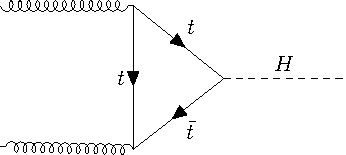
\includegraphics[width=1.1\textwidth]{../notes/higgs.pdf}
            \end{column}
        \end{columns}
    \end{block}
\end{frame}

\begin{frame}{SM4 with 2HDM Type II}
    \begin{itemize}
        \item A Chiral SM4 not excluded with 2HDM 
        \item Introduce a ``wrong sign" limit to cancel new Higgs couplings
            \begin{align*}
                \kappa_u = -\kappa_{d,l}
            \end{align*}
        \item For $\tan\beta\gg2$, the wrong sign limit yields
            \begin{align*}
                \cos(\beta-\alpha) &= \frac{2}{\tan\beta}, & \cos(\beta-\alpha) &= \sin2\beta
            \end{align*}
        \item These are equivalent in the large $\tan\beta$ limit
        \item Relations allow us to reduce free parameters of SM4$\times$2HDM
        \item Aim to extend 2HDM scans to SM4 and constrain model using flavour observables
    \end{itemize}
\end{frame}

\section{Questions}
\begin{frame}
    \begin{center}
        \vspace{60pt}
        \Huge Any Questions?
    \end{center}
\end{frame}

\end{document}
